% Main manuscript; expanded QRISP evaluation and architecture/training controls.
% Detailed diagnostics are in inverse_supersampling_supplement.tex.
\documentclass[10pt,twocolumn,letterpaper]{article}
\usepackage[margin=0.75in,columnsep=0.25in]{geometry}
\usepackage[T1]{fontenc}
\usepackage{mathptmx}
\usepackage{amsmath,amssymb}
\usepackage{graphicx,booktabs,array,tabularx}
\usepackage{tikz}
\usetikzlibrary{arrows.meta,positioning,calc}
% Restrained, redundant color coding for the vector architecture figure.
\definecolor{aifInk}{RGB}{36,44,52}
\definecolor{aifBlue}{RGB}{37,99,147}
\definecolor{aifViolet}{RGB}{100,77,157}
\definecolor{aifTeal}{RGB}{0,115,112}
\definecolor{aifGold}{RGB}{174,116,38}
\usepackage[font=small,labelfont=bf]{caption}
\usepackage{microtype}
\usepackage[hidelinks]{hyperref}
\hypersetup{pdftitle={AEISU: Tensor Core-Accelerated Inverse Supersampling for Real-Time Game Upscaling},
  pdfauthor={Charles Dale B. Gleason},
  pdfsubject={Inverse supersampling architecture, rendered-content evaluation, and output-head ablation}}
\setlength{\parindent}{1em}
\setlength{\parskip}{0pt}
\setlength{\textfloatsep}{11pt plus 2pt minus 2pt}
\setlength{\floatsep}{10pt plus 2pt minus 2pt}
\setlength{\abovedisplayskip}{6pt plus 2pt minus 1pt}
\setlength{\belowdisplayskip}{6pt plus 2pt minus 1pt}
\setlength{\emergencystretch}{1.2em}
\clubpenalty=10000
\widowpenalty=10000
\brokenpenalty=10000
\renewcommand{\topfraction}{0.9}
\renewcommand{\textfraction}{0.07}
\renewcommand{\floatpagefraction}{0.8}
\renewcommand{\dbltopfraction}{0.9}
\renewcommand{\dblfloatpagefraction}{0.55}
\setcounter{dbltopnumber}{3}
\newcommand{\model}{AEISU}
\newcommand{\R}{\mathbb{R}}
\newcommand{\A}{\mathcal{A}}
\newcommand{\U}{\mathcal{U}}
\newcommand{\PS}{\mathcal{S}}
\newcommand{\Cat}{\operatorname{cat}}
\newcommand{\sgn}{\operatorname{sgn}}
\newcolumntype{Y}{>{\raggedright\arraybackslash}X}
\tikzset{block/.style={draw,thin,align=center,minimum height=9mm,font=\small,inner sep=3pt},
  flow/.style={-{Latex[length=1.8mm]},thin},
  tinyblock/.style={draw,thin,align=center,font=\scriptsize,inner sep=3pt}}

\begin{document}
\raggedbottom
\twocolumn[{
\begin{center}
  {\LARGE\bfseries AEISU: Tensor Core-Accelerated Inverse Supersampling\\[2pt]
  for Real-Time Game Upscaling\par}
  \vspace{8pt}
  {\small Charles Dale B. Gleason}\par
  {\small\itshape Independent Researcher}\par
  \vspace{5pt}
  {\footnotesize Draft, 21 October 2026.}\par
  {\scriptsize Copyright 2026 Charles Dale B. Gleason. \href{https://creativecommons.org/licenses/by/4.0/}{CC BY 4.0}; third-party imagery excluded.}\par
\end{center}
\vspace{3pt}
\begin{center}\begin{minipage}{0.95\textwidth}
\small\textbf{Abstract.}
We present \model{}, a compact $2\times$ spatial upscaler that predicts adaptive filters below the input grid and reconstructs directly from source RGB.
A fused mixed-FP8/FP16 implementation achieves 0.132 ms median resident latency for 540p-to-1080p and 0.416 ms for 1080p-to-4K on RTX 5090.
Evaluation on 600 QRISP pairs across five environments tests area, bicubic, and independently rendered inputs with and without spatial antialiasing.
The area-trained model leads Area PSNR/SSIM and has lower bright overshoot and ringing than six neural comparators on target-selected isolated edges.
Four neural comparators obtain lower mean Area LPIPS and better bicubic reconstruction; conservative spatial methods have lower edge excursions.
On Native, PSNR falls below bilinear and EASU despite the lowest mean LPIPS, whose lead over the closest methods is unresolved.
A separately DIV2K-trained L1 checkpoint exceeds RepNet and RT4KSR in mean fidelity and LPIPS on four standard bicubic benchmarks, while higher-compute neural models remain ahead.
On the shared backbone, the adaptive head achieves higher FP16 fidelity and smaller FP8 degradation than the tested RGB-residual and depth-to-space heads.\par
\vspace{10pt}
\end{minipage}\end{center}
\vspace{2pt}
}]

\section{Introduction}
\label{sec:intro}
Single-image super-resolution (SISR) estimates a high-resolution (HR) image from a low-resolution (LR) observation.
Because downsampling discards information, reconstruction depends on both image priors and the observation model.
Convolutional, residual, and transformer methods learn this mapping from paired images~\cite{dong2016srcnn,lim2017edsr,liang2021swinir}.

We focus on \emph{inverse supersampling} for resolved game frames.
A common 8K master is independently area-resolved to a 1080p observation and a 4K target.
The objective is to reconstruct the 4K resolve from the 1080p observation.
This sampling model differs from bicubic image reduction and from rendering a scene independently at two resolutions.

At 1080p input, even narrow full-LR feature maps incur substantial arithmetic and memory traffic.
\model{} keeps convolutional features below the LR grid and uses them to predict adaptive filters applied to the original RGB samples.
Its channel widths, layouts, and precision schedule are designed for Tensor Core convolution; the local RGB reconstruction uses conventional CUDA arithmetic.
We measure the complete resident image-to-image operation, since operation counts alone do not determine latency~\cite{wan2024span,ren2024ntire,nvidia2023gemm}.

Our contributions are:
\begin{enumerate}
  \setlength{\itemsep}{1pt}\setlength{\parskip}{0pt}
  \item source-conditioned polyphase reconstruction with convolutional feature processing below the input grid;
  \item folded mixed-precision execution, with output-head, core-architecture, and training-degradation controls;
  \item multi-condition game evaluation characterizing degradation sensitivity, distortion, and LPIPS perceptual distance.
\end{enumerate}

\section{Related Work}
\label{sec:related}
\paragraph{Learned and efficient image super-resolution.}
SRCNN, ESPCN, EDSR, and SwinIR represent convolutional mapping, LR-grid subpixel reconstruction, residual learning, and transformer restoration, respectively~\cite{dong2016srcnn,shi2016espcn,lim2017edsr,liang2021swinir}.
Their bicubic evaluations use a different observation model from our supersample-resolve task.
Efficient SR methods also emphasize measured execution: SPAN reports quality, latency, and model complexity, while NTIRE evaluates these quantities under common protocols~\cite{wan2024span,ren2024ntire}.
RepNet uses a reparameterized convolutional design for real-time $4\times$ reconstruction~\cite{conde2023repnet}.
RT4KSR reduces deep-feature resolution using pixel unshuffle and structural reparameterization~\cite{zamfir2023rt4ksr}.
QuickSRNet targets real-time mobile upscaling and robustness to quantization~\cite{berger2023quicksrnet}.

\paragraph{Adaptive reconstruction.}
Learned filtering is established in RAISR~\cite{romano2016raisr}.
LAPAR predicts coefficients over predefined Gaussian/DoG bases and applies assembled filters to a bicubic-upsampled image~\cite{li2021lapar}.
Deep Adaptive Image Resampling predicts spatially varying kernels, and DUF predicts upsampling filters from video neighborhoods together with a separate residual~\cite{jia2017adaptive,jo2018duf}.
Kernel Prediction Networks also reconstruct directly from source samples, in their case for burst denoising~\cite{mildenhall2018kpn}.
HDRNet and deep guided filtering couple lower-resolution prediction to source-guided image processing~\cite{gharbi2017hdrnet,wu2018guided}.
\model{} uses a single image, a learned four-phase base, sixteen normalized zero-DC components, and shared RGB weights.
Its distinction is the combination of below-LR prediction, packed source-grid polyphase synthesis, and fused stage-specific precision within this established filtering approach.

\paragraph{Spatial game upscaling.}
FSR1, NIS, and SGSR1 use local, edge-adaptive reconstruction rather than temporal history~\cite{amd2021fsr,nvidia2022nis,qualcomm2023gsr}.
Their integration and reconstruction constraints differ from learned image-restoration models; we include these spatial methods to evaluate that distinct operating regime.

\paragraph{Reparameterization and rendered content.}
Structural reparameterization adds training capacity while retaining a compact inference graph, as in RepVGG~\cite{ding2021repvgg}.
\model{} folds its kernel-space training coordinates into the deployed operators.
QRISP and GameIR provide rendered-content evaluation settings~\cite{mercier2023qrisp,zhou2024gameir}.
Unlike common-master resolves, independently rendered LR/HR frames can differ in shading, level of detail, postprocessing, and aliasing; we evaluate these pairing regimes separately.

\section{Inverse Supersampling Task}
\label{sec:task}
Let $L\in\R^{H\times W\times3}$ denote the observation and $T\in\R^{2H\times2W\times3}$ its reference target.
Let $S\in\R^{4H\times4W\times3}$ be the common master.
For the primary setting, $S$ is $7680\times4320$, $T$ is $3840\times2160$, and $L$ is $1920\times1080$ (width by height).

Define aligned integer-area reduction by $s$ per axis as
\begin{equation}
 \A_s(X)[i,j,c]=\frac{1}{s^2}
 \sum_{u=0}^{s-1}\sum_{v=0}^{s-1}X[si+u,sj+v,c].
 \label{eq:area}
\end{equation}
In ideal arithmetic the pair is
\begin{equation}
 T=\A_2(S),\qquad L=\A_4(S),\qquad \A_2(T)=L.
 \label{eq:task}
\end{equation}
The last identity requires aligned, nested averaging cells and a common numeric domain.
Stored images instead have $T=Q_T(\A_2(S))$ and $L=Q_L(\A_4(S))$, where $Q_T$ and $Q_L$ represent quantization and clipping.
Independent rounding introduces a measurable baseline discrepancy in $\A_2(T)-L$.

We seek an estimator $\widehat T=f_\theta(L)$ fitted to this distribution of pairs.
Area averaging removes spatial information, so resolve consistency alone does not identify $T$.
Evaluation therefore measures HR reconstruction rather than LR consistency alone.

\paragraph{Scope and color domain.}
We distinguish \emph{supersample resolves} of rasterized masters from \emph{integer-area downsampling} of natural images: the averaging operator is the same, but the source distributions differ.
Antialiased bicubic reduction defines a different reconstruction problem.
Area reduction represents a box-filtered footprint, whereas antialiased bicubic uses a different reconstruction kernel~\cite{pharr2023pbrt,mathworksresize}.
The intended input is already antialiased, tone-mapped, perceptually encoded RGB in $[0,1]$.
\model{} includes no dedicated antialiasing or tone-mapping stage.
This placement follows FSR~1's integration contract; GSR~1 also recommends antialiased input for best results~\cite{amd2021fsr,qualcomm2023gsr}.
Independently rendered LR frames provide a transfer evaluation outside the sampling model in Eq.~\eqref{eq:task}.
Encoded-RGB area averaging is not equivalent to linear-light integration; the transfer function, stored range, and resolve ordering affect the observation model.
Section~\ref{sec:data} describes training acquisition and its limitations.

\section{Architecture}
\label{sec:method}
\subsection{Overview and notation}
Figure~\ref{fig:architecture} summarizes the controller and reconstruction path.
\model{} maps $L$ to eight analysis channels, packs spatial samples into channels, and predicts reconstruction coefficients with a multiresolution convolutional controller.
All its feature-map convolutions operate at $H/2\times W/2$ or $H/4\times W/4$.
Analysis arithmetic and reconstruction still operate at the input grid and output phases.
Dimensions not divisible by four are handled by padding and cropping.

Let $\U_2$ denote pixel unshuffle (space-to-depth by two), $\PS_2$ its pixel-shuffle inverse, and $\sigma(x)=\max(x,0)+0.1\min(x,0)$.
Pixel unshuffle rearranges samples without averaging them.
We write $C^{k}_{a\rightarrow b}$ for an affine $k\times k$ convolution with $a$ input and $b$ output channels.
The controller uses unit stride, biases, and zero padding for spatial convolutions.
The analysis stencils and final reconstruction use replicated source borders.
Spatial coordinates and offsets use row--column order, consistent with $\phi=(\phi_y,\phi_x)$.

\begin{figure*}[t]
\centering
\begingroup
% Original vector artwork. Tensor dimensions are annotated, not drawn to scale.
\pgfdeclarelayer{aifWires}
\pgfdeclarelayer{aifEdges}
\pgfsetlayers{aifWires,main,aifEdges}
\newcommand{\aifTensor}[7]{%
  \begin{scope}[shift={(#2,#3)}]
    \path[fill=#7!14]
      (0,0) rectangle (#4,#5);
    \path[fill=#7!25]
      (0,#5)--(#6,{#5+0.65*#6})--({#4+#6},{#5+0.65*#6})--(#4,#5)--cycle;
    \path[fill=#7!36]
      (#4,0)--({#4+#6},{0.65*#6})--({#4+#6},{#5+0.65*#6})--(#4,#5)--cycle;
    \foreach \i in {1,2,3}
      \draw[#7!45,line width=0.3pt]
        ({#4+\i*#6/4},{\i*0.65*#6/4})--({#4+\i*#6/4},{#5+\i*0.65*#6/4});
    % Opaque perimeter strokes cover stripes and crossing connectors.
    % Rounded joins avoid the spikes produced by acute mitered corners.
    \begin{pgfonlayer}{aifEdges}
      \draw[#7!80,line width=0.55pt,line join=round,line cap=round]
        (0,0)--(#4,0)--({#4+#6},{0.65*#6})
        --({#4+#6},{#5+0.65*#6})--(#6,{#5+0.65*#6})--(0,#5)--cycle;
      \draw[#7!80,line width=0.55pt,line join=round,line cap=round]
        (0,#5)--(#4,#5)--(#4,0)
        (#4,#5)--({#4+#6},{#5+0.65*#6});
    \end{pgfonlayer}
    \coordinate (#1-in) at (0,{#5/2});
    \coordinate (#1-out) at ({#4+#6},{#5/2});
    \coordinate (#1-top) at ({#4/2+#6},{#5+0.65*#6});
    \coordinate (#1-bottom) at ({#4/2},0);
  \end{scope}}
\newcommand{\aifGrid}[5]{%
  \begin{scope}[shift={(#1,#2)}]
    \fill[#5!7] (0,0) rectangle (#3,#3);
    \foreach \i in {0,...,#4} {
      \draw[#5!65,line width=0.35pt] ({\i*#3/#4},0)--({\i*#3/#4},#3);
      \draw[#5!65,line width=0.35pt] (0,{\i*#3/#4})--(#3,{\i*#3/#4});
    }
  \end{scope}}
\newcommand{\aifImage}[4]{%
  \begin{scope}[shift={(#1,#2)},x=#3cm,y=#4cm]
    \fill[aifBlue!9] (0,0) rectangle (1,1);
    \fill[aifTeal!25] (0,0)--(0,0.45)--(0.4,0.8)--(0.74,0.29)--(1,0.63)--(1,0)--cycle;
    \fill[aifTeal!55] (0,0)--(0,0.24)--(0.6,0.6)--(1,0.14)--(1,0)--cycle;
    \fill[aifGold!65] (0.8,0.83) circle (0.075);
    \draw[white,line width=1.3pt] (0.18,0)--(0.33,0.26)--(0.54,0.36)--(0.44,0.47);
    \draw[aifInk!65,line width=0.55pt] (0,0) rectangle (1,1);
  \end{scope}}
\resizebox{\textwidth}{!}{%
\begin{tikzpicture}[x=1cm,y=1cm,
  font=\rmfamily\fontsize{9}{10.5}\selectfont,text=aifInk,
  stream/.style={-{Latex[length=1.7mm,width=1.25mm]},draw=aifInk,line width=0.7pt},
  parameter/.style={stream,dashed,draw=aifGold},
  joint/.style={draw=aifInk,fill=white,circle,minimum size=4.5mm,inner sep=0pt},
  note/.style={font=\rmfamily\fontsize{8.1}{9.5}\selectfont,align=center},
  heading/.style={anchor=west,font=\rmfamily\bfseries\fontsize{10}{12}\selectfont}]
\path[use as bounding box] (-0.15,-0.1) rectangle (19.0,12.7);
\node[heading] at (0,12.43) {(a) Neural controller and adaptive RGB reconstruction};
\node[note,anchor=east] at (18.8,12.43) {$H,W$: LR image dimensions};
% Overview/detail hierarchy follows SR-paper conventions; artwork is original.
\begin{pgfonlayer}{aifWires}
  \fill[aifBlue!3,rounded corners=2mm] (3.70,8.88) rectangle (17.60,12.13);
  \fill[aifTeal!3,rounded corners=2mm] (0.02,0.16) rectangle (6.80,5.73);
  \fill[aifGold!3,rounded corners=2mm] (7.30,0.16) rectangle (18.82,5.73);
\end{pgfonlayer}

% Feature volumes shrink spatially, split into independent streams, then expand.
\fill[aifViolet!4,rounded corners=2mm] (6.9,9.00) rectangle (9.85,11.84);
\draw[aifViolet!55,dashed,rounded corners=2mm,line width=0.5pt]
  (6.9,9.00) rectangle (9.85,11.84);
\def\aifThumbWidth{1.10}
\def\aifThumbHeight{1.10}
\aifImage{0.05}{9.70}{\aifThumbWidth}{\aifThumbHeight}
\node[note,anchor=north,inner sep=0pt] at (0.6,9.49) {\textbf{LR RGB} $L$\\[2pt]$H\times W\times3$};
\draw[stream] (1.15,10.25)--(1.86,10.25);
\aifTensor{analysis}{1.9}{9.52}{0.6}{1.47}{0.36}{aifTeal}
% Eight analysis planes: three color mixtures, one luma mixture, four stencils.
\foreach \y in {9.72,9.89,10.06,10.23,10.40,10.57,10.74}
  \draw[aifTeal!45,line width=0.35pt] (1.9,\y)--(2.5,\y);
\node[note] at (2.38,11.56) {\textbf{Learned analysis}\\RGB mix + luma + 4 edges};
\node[note] at (2.38,9.17) {$H\times W\times8$};
\aifTensor{enc}{4.05}{9.72}{0.48}{1.06}{0.32}{aifBlue}
\draw[stream] (analysis-out)--node[above=3pt,note] {$\U_2$\\$1\times1$} (enc-in);
\node[note] at (4.43,9.17) {\textbf{Project}\\$H/2,\;32$};
\aifTensor{cmp}{5.75}{9.93}{0.44}{0.64}{0.32}{aifViolet}
\draw[stream] (enc-out)--node[above=3pt,note] {$\U_2$\\$1\times1$} (cmp-in);
\node[note] at (6.14,9.17) {\textbf{Compress}\\$H/4,\;64$};
\coordinate (split) at (6.72,10.25);
\draw (cmp-out)--(split);
\fill[aifInk] (split) circle (1.1pt);
\foreach \j/\y in {A/10.62,B/9.42} {
  \foreach \i in {0,1,2,3} {
    \pgfmathsetmacro{\xx}{7.12+0.63*\i}
    \aifTensor{b\j\i}{\xx}{\y}{0.25}{0.64}{0.12}{aifViolet}
    \ifnum\i>0
      \pgfmathtruncatemacro{\prev}{\i-1}
      \draw[stream] (b\j\prev-out)--(b\j\i-in);
    \fi
  }
  \draw[stream] (split)|-(b\j0-in);
}
\node[note] at (8.37,11.61) {$4\times[3\times3,\;32\rightarrow32]$};
\node[note] at (8.37,10.34) {Branch A};
\node[note] at (8.37,9.25) {Branch B};
\node[joint,note] (cat) at (10.25,10.25) {C};
\draw[stream] (bA3-out)-|(cat.north);
\draw[stream] (bB3-out)-|(cat.south);
\aifTensor{exp}{11.7}{9.72}{0.46}{1.06}{0.3}{aifViolet}
\draw[stream] (cat)--node[above=3pt,note] {$1\times1$\\$\PS_2$} (exp-in);
\node[note] at (11.98,9.17) {\textbf{Expand}\\$H/2,\;32$};
\node[joint,font=\large] (add) at (12.94,10.25) {$+$};
\draw[stream] (exp-out)--(add);
% The long skip carries only half-resolution features, never reconstructed RGB.
\begin{pgfonlayer}{aifWires}
  \draw[stream,draw=aifBlue] (enc-top)--(enc-top |- 0,11.95)--(12.94,11.95)--(add.north);
\end{pgfonlayer}
\node[note,fill=aifBlue!3,inner sep=1.5pt,text=aifBlue] at (10.75,11.95)
  {$H/2$ feature skip};
\aifTensor{ref}{14.0}{9.72}{0.46}{1.06}{0.46}{aifBlue}
\draw[stream] (add)--node[above=3pt,note] {$3\times3$} (ref-in);
\node[note] at (14.45,9.17) {\textbf{Refine}\\$H/2,\;64$};
\aifTensor{head}{16.3}{9.72}{0.66}{1.06}{0.45}{aifTeal}
\draw[stream] (ref-out)--node[above=3pt,note] {$1\times1$\\linear} (head-in);
\node[note] at (16.85,11.43) {\textbf{Packed coefficients} $V$};
\node[note] at (16.85,9.17) {$H/2\times W/2\times64$\\$4$ LR sites $\times16$ coefficients};
% Each output pixel is reconstructed from original samples, not decoded RGB.
\fill[aifInk] (1.48,10.25) circle (1.1pt);
\draw[stream,line width=0.8pt] (1.48,10.25)--(1.48,7.825)--(14.68,7.825);
\node[note,fill=white,inner sep=2pt] at (6.45,7.825)
  {\textbf{Original RGB samples}};
\draw[stream,draw=aifTeal] (head-out)--(18.96,10.25)--(18.96,8.68)--(15.175,8.68)--(15.175,8.32);
\aifGrid{14.8}{7.45}{0.75}{5}{aifGold}
\aifGrid{16.3}{7.45}{0.75}{2}{aifGold}
\draw[stream] (15.67,7.825)--(16.18,7.825);
\node[note,anchor=north,inner sep=0pt] at (15.97,6.95)
  {\textbf{Fused filter head}};
\draw[parameter] (13.15,7.15)--(15.175,7.15)--(15.175,7.33);
\node[note,anchor=east,inner sep=0pt] at (12.98,7.15) {Learned base + bank};
\draw[stream] (17.17,7.825)--(17.65,7.825);
\aifImage{17.65}{7.275}{\aifThumbWidth}{\aifThumbHeight}
\node[note,anchor=north,inner sep=0pt] at (18.20,7.065)
  {\textbf{HR RGB} $\widehat T$\\[2pt]$2H\times2W\times3$};

\draw[aifInk!20,line width=0.5pt] (0,6.16)--(18.85,6.16);
\node[heading] at (0,5.88) {(b) Packed coefficient layout};
\node[heading] at (7.35,5.88) {(c) Source-conditioned reconstruction};

% The packing inset makes LR parity distinct from the reconstruction phases.
\node[note] at (1.8,5.52) {One spatial cell of $V$};
\foreach \x/\col/\lab in {0.32/aifBlue/0,1.07/aifViolet/1,1.82/aifTeal/2,2.57/aifGold/3} {
  \foreach \i in {0,...,15}
    \path[draw=\col!65,fill=\col!18,line width=0.25pt]
      (\x,{3.99+0.07*\i}) rectangle ({\x+0.5},{4.06+0.07*\i});
  \node[note] at ({\x+0.25},3.74) {$\lab$};
}
\node[note] at (1.7,3.31) {Parity $\rho$: four groups of 16};
\draw[stream] (3.18,4.56)--node[above,note] {index} (4.23,4.56);
\foreach \x/\y/\col/\lab in {4.38/4.56/aifBlue/0,5.06/4.56/aifViolet/1,4.38/3.88/aifTeal/2,5.06/3.88/aifGold/3} {
  \path[draw=\col,fill=\col!16,line width=0.65pt]
    (\x,\y) rectangle ({\x+0.68},{\y+0.68});
  \node[note] at ({\x+0.34},{\y+0.34}) {$\lab$};
}
\node[note] at (5.07,5.52) {$2\times2$ LR sites, parity $\rho$};
\node[note] at (5.07,3.31) {Read the selected\\16-channel group};
\draw[stream] (5.86,4.91)--(6.29,4.91)--(6.29,2.86);
\node[note,fill=white,inner sep=2pt] at (6.29,3.49) {$g$};
\foreach \i in {0,...,15}
  \path[draw=aifTeal!70,fill=aifTeal!14,line width=0.35pt]
    ({0.4+0.38*\i},2.22) rectangle ({0.78+0.38*\i},2.7);
\node[note,anchor=north west,inner sep=0pt] at (0.4,2.08) {$a_0$};
\node[note,anchor=north,inner sep=0pt] at (3.44,2.08) {$\cdots$};
\node[note,anchor=north east,inner sep=0pt] at (6.48,2.08) {$a_{15}$};
\node[note] at (3.43,1.51) {\textbf{16 coefficients} $a_p$ for LR site $p$};
\node[note,align=center,text width=6.1cm] at (3.43,0.87)
  {LR-site parity $\rho$ selects a group, not an HR phase.\\No full-LR coefficient tensor is materialized.};

% A parameter bank, a four-phase spatial footprint, and a source-patch dot product.
\node[note] at (8.27,5.52) {Bank $K$};
\aifGrid{8.02}{4.48}{0.84}{5}{aifGold}
\aifGrid{7.90}{4.36}{0.84}{5}{aifGold}
\aifGrid{7.78}{4.24}{0.84}{5}{aifGold}
\node[note] at (8.28,4.01) {$K_{0,\phi},\ldots,K_{15,\phi}$};
\aifGrid{7.78}{2.86}{0.84}{5}{aifGold}
\node[note] at (8.23,2.59) {Learned base $B_\phi$};
\node[joint,font=\large] (mix) at (9.65,3.75) {$+$};
\node[joint] (weighted) at (9.65,4.85) {$\Sigma$};
\draw[stream] (8.95,4.68)--(9.23,4.68)|-(weighted.west);
\draw[stream] (weighted.south)--(mix.north);
\draw[stream] (9.65,5.44)--(weighted.north);
\node[note] at (9.65,5.62) {$a_p$};
\draw[stream] (8.65,3.28)-|(mix.south);
\draw[stream] (mix)--(10.34,3.75);
\foreach \x/\y/\u/\v in {10.45/4.17/0/0,11.75/4.17/0/1,10.45/2.77/1/0,11.75/2.77/1/1} {
  \aifGrid{\x}{\y}{0.94}{5}{aifGold}
  \node[note,anchor=north,inner sep=0pt] at ({\x+0.47},{\y-0.12}) {$(\u,\v)$};
}
\node[note] at (11.56,5.52) {$W_{p,\phi}$: phases $(\phi_y,\phi_x)$};
\node[note,anchor=west,align=left] at (13.48,4.75)
  {\textbf{Four $5\times5$ filters}\\One per HR phase\\Shared across R, G, B};
\node[note,anchor=west,align=left,text width=4.7cm] at (13.48,3.6)
  {$W_{p,\phi}=B_\phi+\sum_{k=0}^{15}a_{p,k}K_{k,\phi}$\\[4pt]
   Fused filter assembly\\and RGB reconstruction.\\No image-sized filter buffer.};
% Pixel geometry: center LR site and the corresponding 2x2 HR block.
\aifGrid{8.03}{0.54}{1.45}{5}{aifInk}
\fill[aifGold!45] (8.61,1.12) rectangle (8.9,1.41);
\fill[aifInk] (8.755,1.265) circle (0.6pt);
\draw[aifInk!65,line width=0.45pt] (8.69,1.20)--(7.73,0.55);
\node[note,anchor=north east,inner sep=0pt] at (7.71,0.53) {$p$};
\node[note,anchor=west,align=left] at (9.77,0.81)
  {$5\times5$ original\\RGB neighborhood};
\node[joint,font=\large] (dot) at (13.63,1.65) {$\cdot$};
\draw[stream] (9.51,1.65)--(dot.west);
\draw[stream] (12.87,4.58)--(13.14,4.58)--(13.14,2.24)--(13.63,2.24)--(dot.north);
\node[note] at (14.34,2.14) {$\sum_\delta$};
\draw[stream] (dot.east)--(15.02,1.65);
\foreach \x/\y/\u/\v in {15.14/1.5/0/0,15.87/1.5/0/1,15.14/0.77/1/0,15.87/0.77/1/1} {
  \path[draw=aifGold,fill=aifGold!13,line width=0.65pt]
    (\x,\y) rectangle ({\x+0.73},{\y+0.73});
  \node[font=\rmfamily\fontsize{7.5}{9}\selectfont,
    inner sep=0pt,text height=1.7mm,text depth=0.7mm]
    at ({\x+0.365},{\y+0.365}) {$(\u,\v)$};
}
\node[note,anchor=south,inner sep=0pt] at (15.87,2.4) {Phase $(\phi_y,\phi_x)$};
\node[note,anchor=west,align=left] at (16.86,1.5)
  {\textbf{$2\times2$ HR}\\RGB pixels\\$\widehat T(2p+\phi)$};
\end{tikzpicture}}
\endgroup

\caption{\textbf{Inference architecture.} \textbf{(a)} Learned analysis feeds two quarter-resolution branches and a half-resolution skip; original RGB samples bypass the controller. \textbf{(b)} The head packs sixteen coefficients for each of four LR-site parities, followed by clamp $g$. \textbf{(c)} Each coefficient vector combines the learned base and bank into four $5\times5$ phase filters applied to the source RGB neighborhood. Filter assembly and reconstruction are fused. $\U_2$: pixel unshuffle; $\PS_2$: pixel shuffle; C: concatenate. Convolutions use LeakyReLU$(0.1)$ except the linear head. Tensor sizes are annotated; icons are schematic.}
\label{fig:architecture}
\end{figure*}

\subsection{Learned analysis inputs}
\label{sec:analysis}
For a source RGB vector $l(p)\in\R^3$, a learned matrix $M\in\R^{3\times3}$ forms three transformed color channels,
\begin{equation}
 z(p)=M l(p),\qquad y(p)=m^\mathsf{T}l(p),\quad m\in\R^3.
 \label{eq:analysis}
\end{equation}
The scalar $y$ is a learned color mixture initialized with luminance weights.
$M$ is initialized to identity, and $m$ is initialized to $(0.2126,0.7152,0.0722)$.
Four learned, zero-sum directional $3\times3$ stencils produce responses $d_x,d_y,d_{45},d_{135}$ from $y$.
For example,
\begin{equation}
 d_x(p)=\sum_{j=-1}^{1}\alpha_{j+1}
 \big[y(p+(j,1))-y(p+(j,-1))\big].
 \label{eq:dx}
\end{equation}
The remaining operators exchange or combine axis and diagonal differences (Supplementary Material, Section~S1).
Each starts with a Sobel-like response and learns three parameters controlling directional weighting and strength.
The feature pack is
\begin{equation}
 E(p)=\big[z_1,z_2,z_3,y,d_x,d_y,d_{45},d_{135}\big](p).
 \label{eq:pack}
\end{equation}
The analysis uses 24 global learned parameters.
Native execution fuses analysis with the packed projection; the RGB transform can be absorbed into its weights.
Reconstruction still samples the original RGB image $L$.
Section~\ref{sec:core-controls} evaluates a frozen-analysis control.

\subsection{Controller below the input resolution}
The half-resolution encoding is
\begin{equation}
 F_{1/2}=\sigma\big(C^1_{32\rightarrow32}(\U_2(E))\big),
 \label{eq:enc}
\end{equation}
and the quarter-resolution encoding is
\begin{equation}
 Z_{1/4}=\sigma\big(C^1_{128\rightarrow64}(\U_2(F_{1/2}))\big).
 \label{eq:compress}
\end{equation}
The dense compression learns how information is distributed into the two subsequent 32-channel branches.
Let $(Z^a_0,Z^b_0)=\operatorname{split}_{32}(Z_{1/4})$.
Each branch has four independently parameterized spatial layers:
\begin{equation}
 Z^j_i=\sigma\big(C^{3,j,i}_{32\rightarrow32}(Z^j_{i-1})\big),
 \quad j\in\{a,b\},\ i=1,\ldots,4.
 \label{eq:branches}
\end{equation}
There is no cross-branch mixing inside these four layers.
Concatenation and a dense expansion mix their final representations:
\begin{align}
 U_{1/2}&=\PS_2\left(\sigma\left(C^1_{64\rightarrow128}
             \big(\Cat(Z^a_4,Z^b_4)\big)\right)\right),\label{eq:expand}\\
 F&=\sigma\big(C^3_{32\rightarrow64}(F_{1/2}+U_{1/2})\big).
 \label{eq:refine}
\end{align}
$F$ is the shared feature tensor used for the output-head ablations.

The branch design preserves the spatial-convolution MAC count of a reference core comprising two $64\rightarrow64$ spatial layers:
\begin{equation}
 2\cdot4\cdot32^2\cdot9
 =2\cdot64^2\cdot9
 =73{,}728
 \label{eq:branchmac}
\end{equation}
MACs per quarter-resolution site.
The split increases depth while retaining two independent feature groups.
Section~\ref{sec:core-controls} compares this deeper, grouped core with the equal-MAC dense alternative.

\subsection{Packed coefficient head}
\label{sec:head}
A linear $1\times1$ head maps $F$ to
\begin{equation}
 V=C^1_{64\rightarrow64}(F)
 \in\R^{H/2\times W/2\times64}.
 \label{eq:head}
\end{equation}
For an LR site $p=(i,j)$, define $q=(\lfloor i/2\rfloor,\lfloor j/2\rfloor)$ and
$\rho(p)=2(i\bmod2)+(j\bmod2)$.
The raw coefficient vector is indexed directly from the packed head:
\begin{equation}
 \widetilde a_{p,k}=V[q,16\rho(p)+k],\qquad k=0,\ldots,15.
 \label{eq:parity}
\end{equation}
$\rho$ identifies an \emph{input-site parity} within a $2\times2$ LR block.
It is distinct from the four \emph{output phases} generated for each individual LR site.
The runtime can use this indexing directly, without materializing a full-resolution coefficient image.

A symmetric soft coefficient clamp maps raw predictions to $a_{p,k}=g(\widetilde a_{p,k})$:
\begin{equation}
 g(t)=\sgn(t)\begin{cases}
 |t|, & |t|\leq2,\\
 2+0.05(|t|-2), & 2<|t|\leq12,\\
 2.5, & |t|>12.
 \end{cases}
 \label{eq:coefficient-clamp}
\end{equation}
Coefficients pass unchanged within $[-2,2]$, grow with slope $0.05$ beyond this interval, and saturate at $\pm2.5$.
The clamp bounds adaptive modulation; it does not constrain reconstructed RGB to the local source range.
Section~\ref{sec:clamp-ablation} compares this transfer with unrestricted coefficients.

\subsection{Polyphase reconstruction}
\label{sec:reconstruct}
Let $\mathcal D=\{-2,-1,0,1,2\}^2$ be the $5\times5$ LR support, and let $\phi=(\phi_y,\phi_x)\in\{0,1\}^2$ identify the four HR phases.
The model stores a learned base $B_\phi[\delta]$ and sixteen adaptive components $K_{k,\phi}[\delta]$.
For each LR site it synthesizes
\begin{equation}
 W_{p,\phi}[\delta]=B_\phi[\delta]
             +\sum_{k=0}^{15}a_{p,k}K_{k,\phi}[\delta].
 \label{eq:kernel}
\end{equation}
The output is
\begin{equation}
 \widehat T[2p+\phi,c]
   =\sum_{\delta\in\mathcal D}W_{p,\phi}[\delta]\,
     L[\pi(p+\delta),c],
 \label{eq:reconstruct}
\end{equation}
where $\pi$ clamps an out-of-bounds coordinate to the image border.
One coefficient vector controls all four output phases.
The synthesized spatial weights are shared across the three RGB channels, although the coefficient predictor observes color information.
The adaptive bank contains $16\cdot4\cdot25=1{,}600$ values and the base contains $4\cdot25=100$.

For each component and phase, the effective kernel is obtained from an unconstrained vector $D_{k,\phi}$ by
\begin{align}
 \bar D_{k,\phi}[\delta]
 &=D_{k,\phi}[\delta]-\frac1{25}\sum_{\delta'}D_{k,\phi}[\delta'],\\
 K_{k,\phi}[\delta]
 &=\lambda\frac{\bar D_{k,\phi}[\delta]}
 {\max\!\left(\sum_{\delta'}|\bar D_{k,\phi}[\delta']|,\epsilon\right)},
 \label{eq:projection}
\end{align}
with $\lambda=0.5$ and $\epsilon=10^{-6}$.
Each effective component has zero DC response and $\ell_1$ norm at most $0.5$ in exact arithmetic; its taps may be signed.

\smallskip
\noindent\begin{minipage}[t]{0.69\linewidth}
\vspace{0pt}
\textbf{Learned upscale base.} The four $5\times5$ base kernels start as bilinear $2\times$ sampling with half-pixel coordinates and remain trainable.
The zero-initialized coefficient head makes the initial output bilinear.
Learning adapts these phase-filter constants without changing their support.
Its weights enter Eq.~\eqref{eq:kernel} directly, so deployment does not evaluate a separate base image.
\end{minipage}\hfill
\begin{minipage}[t]{0.28\linewidth}
\vspace{2pt}\centering
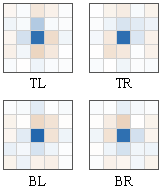
\includegraphics[width=\linewidth]{figures/learned_base_inset.pdf}\par
{\fontsize{6.5}{7.5}\selectfont Learned base phases\\Blue: $+$; orange: $-$}\par
\end{minipage}\par\smallskip

Zero DC suppresses the adaptive term on constant neighborhoods, while the learned base remains unconstrained.
Supplementary Material, Sections~S2 and S6, provides a coefficient-perturbation bound and a bank visualization; Section~\ref{sec:ablation} tests quantization robustness.

\begin{table*}[t]
\centering\small
\caption{Deployed controller dimensions and convolution MACs per input pixel. Shapes omit the batch dimension. LeakyReLU follows each convolution except the linear coefficient head. Counts cover convolution only.}
\label{tab:shapes}
\begin{tabular}{llllr}
\toprule
Stage & Operation & Spatial size & Channels & MACs / LR pixel\\
\midrule
Analysis & Learned color mixtures and directional stencils & $H\times W$ & $3\to8$ & ---\\
Encoding & $\U_2$; $1\times1$ projection & $H/2\times W/2$ & $32\to32$ & 256\\
Compression & $\U_2$; $1\times1$ projection & $H/4\times W/4$ & $128\to64$ & 512\\
Parallel core & Two branches, four $3\times3$ layers each & $H/4\times W/4$ & $2\times(32\to32)$ & 4,608\\
Expansion & $1\times1$ projection; $\PS_2$ & $H/4\to H/2$, $W/4\to W/2$ & $64\to128\to32$ & 512\\
Refinement & Skip addition; $3\times3$ convolution & $H/2\times W/2$ & $32\to64$ & 4,608\\
Coefficient head & Linear $1\times1$ projection & $H/2\times W/2$ & $64\to64$ & 1,024\\
\midrule
Controller total & 13 deployed convolutions & & & 11,520\\
\bottomrule
\end{tabular}
\end{table*}

\subsection{Training-time reparameterization}
Training adds parameter branches to convolution weights, input analysis, the base, and the adaptive bank, then folds them into the deployed operators.
The bank's 64 temporary four-phase kernels and $64\times16$ mixing matrix assemble the same sixteen effective components before normalization.
These training-only coordinates introduce no additional image-sized inference branches and preserve the deployed architecture.
Supplementary Material gives the kernel-space folding maps.

\section{Tensor Core-Oriented Inference}
\label{sec:runtime}
\subsection{Shape and work placement}
The convolutional controller uses widths 32, 64, and 128 to support regular matrix tiling on Tensor Cores.
The reduction dimensions are $C_{\rm in}$ for $1\times1$ convolution and $9C_{\rm in}$ for $3\times3$ convolution.
Actual throughput also depends on datatype, occupancy, kernel implementation, and data movement~\cite{nvidia2023gemm}.

Table~\ref{tab:shapes} gives $11{,}520HW$ convolution MACs.
For $1920\times1080$ input this is $23.887872$ billion MACs.
The production representation stores 115,996 scalars: 113,664 convolution weights, 608 biases, 24 analysis parameters, and 1,700 reconstruction values.
Training-only coordinates and quantization metadata are excluded; folding the color transform into the first projection changes the equivalent stored representation.

\subsection{Fused reconstruction and mixed precision}
Equation~\eqref{eq:kernel} permits the learned base and adaptive contribution to be accumulated together.
The implementation reuses a local RGB neighborhood across output phases and RGB channels, consumes coefficients from the packed head, and stores shared kernel components in a layout convenient for phase-wise access.
The conventional-CUDA reconstruction stage assembles and applies filters without writing an image-sized kernel buffer to global memory.

Numerical formats are selected by stage to balance arithmetic, conversion, and memory costs.
The mixed-precision configuration uses FP16 analysis/projection and a fused FP16 refinement/head, with FP8 E4M3 operands in compression, the parallel core, and expansion.
Reconstruction remains a separate non-FP8 operator.
Precision labels refer to operands and stored intermediates; controller accumulation uses FP32.
Section~\ref{sec:precision} describes calibration.

\section{Experimental Evaluation}
\label{sec:eval}
\subsection{Training data and optimization}
\label{sec:data}
Training uses 700 frames selected from $7680\times4320$ game captures: 635 from \emph{Honkai: Star Rail} and 65 from \emph{Red Dead Redemption 2}.
Frames were selected by a pixel-diversity heuristic and area-resolved to $1920\times1080$ inputs and $3840\times2160$ targets.
The documented Star Rail recording pipeline uses OBS and NVENC AV1, rather than lossless renderer buffers.
Capture settings and the incomplete historical acquisition record are described in Supplementary Material, Section~S3.

The primary model was trained from fresh initialization for 1,000 epochs (875,000 updates), with batch 32, aligned $512\times512$ HR crops, $256\times256$ LR content, and a 16-pixel LR context border.
Each epoch comprises 875 random-crop batches (28,000 sampled patches).
Augmentation samples the eight $D_4$ transforms: rotations by multiples of $90^\circ$ and reflections.
RGB MSE is optimized with AdamW ($\beta=(0.9,0.999)$, $\epsilon=10^{-8}$, zero weight decay), gradient-norm clipping at 1, and cosine decay from $2\times10^{-3}$ to $10^{-6}$ without warmup.
Training uses BF16 AMP, channels-last tensors, and seed 1234.
The adaptive reconstruction uses a custom backward pass: coefficient gradients are evaluated densely, while gradients for the learned base and bank use spatial subsampling at LR-grid stride 16.
Supplementary Material specifies the sampling policy.
We use the final epoch, without validation-based checkpoint selection.
Section~\ref{sec:ablation} uses separate 100-epoch architecture controls and a 1,000-epoch bicubic-training control.

\subsection{Expanded QRISP protocol}
\label{sec:luma-games}
We evaluate 600 supplied $960\times540$/$1920\times1080$ pairs across QRISP's AbandonedSchool, ScifiBaseNightStartStop, ScifiFacility, SeaPort, and SunTempleBush environments~\cite{mercier2023qrisp}.
Each contributes 120 pairs: 40 from each of three area-resolve agreement strata.
Within an environment, pairs are ranked by encoded-Y MSE between supplied LR and floating-point $2\times2$ area-reduced HR, after a four-LR-pixel border crop.
The lowest quarter, middle half, and highest quarter define the most-, middle-, and least-agreement strata.
Uniform rank-quantile sampling within strata and a temporal-spacing guard select frames before inference; 55 source-sequence clusters are represented.
The agreement score responds to texture, aliasing, alignment, and rendering differences.
Equal stratum representation defines a balanced conditional sample rather than a prevalence-weighted QRISP estimate.

Five input conditions share the unchanged Native HR target and frame identities.
SSAA/area uses aligned $2\times2$ averaging of that target, rounded half-up to uint8.
Antialiased bicubic uses Pillow BICUBIC reduction of the same target.
FXAA and SMAA process the supplied Native LR frame; Native applies no additional preprocessing.
The latter three test independently rendered transfer; the first two are common-reference reconstruction controls.
Every method receives identical inputs within each condition, including the same Pillow-bicubic degradation rather than MATLAB resizing.
QRISP's Native color modality is non-jittered with zero mipmap bias; antialiasing and frame-blurring postprocessing are disabled~\cite{mercier2023qrisp}.
FXAA uses NVIDIA 3.11 PC Quality preset 12, subpixel factor 0.75, thresholds 0.166/0.0833, and encoded-RGB luma~\cite{lottes2011fxaa311}.
SMAA uses 1x High, luma edges and lookup textures, with linear-light blending~\cite{jimenez2012smaa}.
Filtered inputs remain floating point.

\paragraph{Comparators and metrics.}
All thirteen methods appear in Table~\ref{tab:final-qrisp}: interpolation, FSR1 EASU with/without RCAS at 0.2 stops, NIS at sharpness 0, SGSR1, RepNet, RT4KSR, QuickSRNet Small/Medium, SPAN, SwinIR-Light, and deployed mixed \model{}.
Spatial/interpolation references use FP32; released neural models use full-frame FP16, without retraining, tiling, or ensembles.
QuickSRNet uses the standard AIMET Model Zoo $2\times$ checkpoints.
Exact checkpoint identities and execution settings are listed in Supplementary Material.

Primary scores are encoded-Y PSNR/SSIM and RGB LPIPS-AlexNet v0.1~\cite{zhang2018lpips}, computed from clipped floating-point outputs after a two-HR-pixel border crop.
For RGB in $[0,1]$,
\begin{equation}
 Y=\frac{65.481R+128.553G+24.966B+16}{255}.
 \label{eq:luma-eval}
\end{equation}
PSNR uses peak 1; SSIM uses an $11\times11$ Gaussian window ($\sigma=1.5$), population moments and the valid interior~\cite{basicsrmetrics,wang2004ssim}.
LPIPS uses full-resolution RGB mapped to $[-1,1]$, without resizing or patch averaging.
RGB PSNR/SSIM and uncropped variants are archived.
Per-image scores are averaged within an environment, then the five environments are weighted equally.
At this evaluation geometry, resident mixed \model{} inference takes $0.132$ ms median ($0.152$ ms p95), measured in the five-trial resolution sweep (Supplementary Material, Section~S5).

A post-hoc paired hierarchical bootstrap resamples environments and source-sequence clusters 50,000 times, preserving pairing.
We report nominal 95\% intervals and approximate simultaneous 95\% standardized-bootstrap bands within separate comparison families.
In the results below, inferential comparisons use simultaneous bands that exclude zero; point-estimate comparisons are identified as means.
Bands containing zero leave the ordering unresolved, without establishing equivalence.
The five-environment sample makes these post-hoc bands exploratory.
Supplementary Material, Section~S4, details comparison families, scene sensitivity, and numerical reproduction.

\begin{table*}[t]
\centering
\caption{Expanded QRISP evaluation: 600 source pairs, five environments, unchanged Native HR targets. P: encoded-Y PSNR (dB, higher is better); S: encoded-Y SSIM (higher); L: RGB LPIPS-AlexNet v0.1 (lower). Scores average per-image values within environments, then weight environments equally. Shader/interpolation baselines use FP32; released neural checkpoints use FP16; \model{} uses deployed mixed precision. All conditions use the same two-HR-pixel border crop.}
\label{tab:final-qrisp}
\begingroup\fontsize{8}{9.5}\selectfont\setlength{\tabcolsep}{3.2pt}
\renewcommand{\arraystretch}{1.0}
\textbf{(a) Common-reference reconstruction controls}\par\smallskip
\begin{tabular}{l*{6}{r}}
\toprule
Method & \multicolumn{3}{c}{SSAA / area} & \multicolumn{3}{c}{Bicubic + AA}\\
\cmidrule(lr){2-4}\cmidrule(lr){5-7}
 & P & S & L & P & S & L\\
\midrule
Bilinear & 28.957 & 0.8602 & 0.2362 & 28.839 & 0.8546 & 0.2610 \\
Bicubic & 29.641 & 0.8841 & 0.2115 & 29.584 & 0.8799 & 0.2370 \\
FSR1 EASU & 29.690 & 0.8820 & 0.1806 & 29.536 & 0.8757 & 0.2117 \\
EASU+RCAS & 29.632 & 0.8892 & 0.1259 & 29.637 & 0.8865 & 0.1505 \\
NIS (0) & 29.621 & 0.8814 & 0.2054 & 29.535 & 0.8766 & 0.2333 \\
SGSR1 & 29.335 & 0.8802 & 0.1456 & 29.351 & 0.8779 & 0.1583 \\
RepNet & 30.148 & 0.8954 & 0.1648 & 30.592 & 0.8969 & 0.1900 \\
RT4KSR & 29.982 & 0.8966 & 0.1461 & 30.693 & 0.9048 & 0.1619 \\
QuickSRNet S & 30.227 & 0.9046 & 0.1066 & 31.527 & 0.9163 & 0.1225 \\
QuickSRNet M & 30.136 & 0.9050 & 0.0985 & 31.838 & 0.9204 & 0.1151 \\
SPAN & 29.462 & 0.9032 & 0.0837 & 32.598 & 0.9290 & 0.0947 \\
SwinIR-Light & 29.575 & 0.9027 & 0.0782 & 32.876 & 0.9324 & 0.0870 \\
\midrule
\model{} mixed & 31.338 & 0.9144 & 0.1120 & 31.062 & 0.9077 & 0.1509 \\
\bottomrule
\end{tabular}
\par\medskip
\textbf{(b) Independently rendered inputs}\par\smallskip
\begin{tabular}{l*{9}{r}}
\toprule
Method & \multicolumn{3}{c}{FXAA input} & \multicolumn{3}{c}{SMAA input} & \multicolumn{3}{c}{Native input}\\
\cmidrule(lr){2-4}\cmidrule(lr){5-7}\cmidrule(lr){8-10}
 & P & S & L & P & S & L & P & S & L\\
\midrule
Bilinear & 27.002 & 0.8091 & 0.3006 & 27.086 & 0.8224 & 0.2754 & 27.292 & 0.8304 & 0.2526 \\
Bicubic & 27.226 & 0.8254 & 0.2722 & 27.148 & 0.8367 & 0.2539 & 27.088 & 0.8405 & 0.2411 \\
FSR1 EASU & 27.271 & 0.8246 & 0.2511 & 27.212 & 0.8364 & 0.2267 & 27.317 & 0.8425 & 0.2040 \\
EASU+RCAS & 27.252 & 0.8316 & 0.1930 & 26.979 & 0.8375 & 0.1776 & 26.898 & 0.8389 & 0.1653 \\
NIS (0) & 27.236 & 0.8237 & 0.2684 & 27.200 & 0.8355 & 0.2482 & 27.233 & 0.8406 & 0.2292 \\
SGSR1 & 27.067 & 0.8246 & 0.1997 & 26.735 & 0.8301 & 0.1916 & 26.680 & 0.8316 & 0.1858 \\
RepNet & 27.346 & 0.8323 & 0.2325 & 26.942 & 0.8407 & 0.2140 & 26.289 & 0.8337 & 0.2167 \\
RT4KSR & 27.251 & 0.8323 & 0.2099 & 26.798 & 0.8377 & 0.1959 & 26.099 & 0.8280 & 0.2048 \\
QuickSRNet S & 27.268 & 0.8362 & 0.1785 & 26.710 & 0.8407 & 0.1680 & 25.822 & 0.8294 & 0.1826 \\
QuickSRNet M & 27.226 & 0.8364 & 0.1729 & 26.588 & 0.8396 & 0.1619 & 25.588 & 0.8260 & 0.1775 \\
SPAN & 27.083 & 0.8357 & 0.1594 & 26.269 & 0.8362 & 0.1494 & 24.032 & 0.8121 & 0.1887 \\
SwinIR-Light & 27.071 & 0.8345 & 0.1567 & 26.287 & 0.8343 & 0.1454 & 25.058 & 0.8146 & 0.1725 \\
\midrule
\model{} mixed & 27.495 & 0.8410 & 0.1899 & 27.139 & 0.8500 & 0.1708 & 26.673 & 0.8473 & 0.1607 \\
\bottomrule
\end{tabular}
\endgroup
\end{table*}

\subsection{Degradation-dependent reconstruction}
Area fidelity is \model{}'s strongest result: mixed inference reaches $31.338$ dB Y PSNR and $0.91436$ SSIM, exceeding every comparator on both metrics.
The PSNR gain over the closest external method, QuickSRNet Small, is $1.111$ dB.
Environment gains range from $0.750$ to $1.554$ dB; omitting any one environment leaves a $1.000$--$1.201$ dB gain.
SwinIR-Light, SPAN, and both QuickSRNet variants nevertheless have lower mean LPIPS.
QuickSRNet Small's mean LPIPS advantage is $0.00537$, with a nominal interval spanning zero.

Bicubic reverses the fidelity ordering: QuickSRNet Small/Medium, SPAN, and SwinIR outperform \model{} on all three metrics.
The adaptive-minus-SwinIR PSNR gap shifts by $-3.577$ dB from area to bicubic (Fig.~\ref{fig:diagnostics}b).
Section~\ref{sec:training-degradation} examines this sensitivity by changing \model{}'s training inputs.
SPAN and SwinIR-Light obtain these LPIPS scores with pixel-loss training~\cite{wan2024span,liang2021swinir,berger2023quicksrnet}.
Mean LPIPS is worse on bicubic than on area for every method; the neural models' relative LPIPS gains arise from smaller deterioration.

FXAA and SMAA inputs give \model{} higher SSIM than every comparator.
It also has the highest mean FXAA PSNR and improves against most comparators; the small SMAA PSNR gaps from several spatial methods remain unresolved.
SPAN/SwinIR have lower mean LPIPS on both conditions, with greater scene dependence on SMAA.
Within \model{}, FXAA raises Native PSNR by $0.822$ dB while worsening LPIPS by $0.02912$.

\subsection{Native transfer and edge reconstruction}
On Native, \model{} has the highest mean SSIM and lowest mean LPIPS, but loses PSNR to EASU by $0.644$ dB (nominal 95\% interval approximately $[-0.785,-0.380]$ dB).
It is also $0.619$ dB below bilinear; every tested learned model has lower mean Native PSNR than bilinear.
The deficit occurs in all five environments and corresponds to approximately 18\% higher arithmetic mean Y MSE.
Conversely, its LPIPS advantage over EASU is $0.04326$, with lower LPIPS on every sampled frame.
The closer mean LPIPS lead over SwinIR is $0.01180$; SwinIR leads two environment means and EASU+RCAS leads SeaPort.

EASU's mean PSNR is only $0.025$ dB above bilinear on Native, yet it improves SSIM by $0.01207$ and LPIPS by $0.04862$.
RCAS improves LPIPS in every condition; on Native it lowers EASU PSNR by $0.419$ dB while narrowing the mean adaptive LPIPS lead to $0.00451$.
Neither this lead nor the lead over SwinIR is resolved by the simultaneous bands.
Supplementary Material, Section~S4.3 reports environment effects and omission sensitivity.
NIS has similar mean distortion scores to EASU on most conditions but worse LPIPS; SGSR1 has lower LPIPS than EASU but often lower PSNR.

\paragraph{Qualitative edge reconstruction.}
Figure~\ref{fig:external-edges} compares selected curved-edge regions from GameIR Town05 using target-derived area inputs.
\model{} shows visibly reduced bright edge halos and ringing relative to the displayed neural comparators, with faint residual fringing and sharper contours than EASU.
An additional GameIR window-surround crop appears in Supplementary Material. These qualitative examples are separate from the QRISP numerical evaluation.

\paragraph{Target-selected edge profiles.}
A complementary diagnostic samples 40,517 isolated-edge profiles in 570 of the 600 targets, independently of model outputs.
On Area, \model{} has 76--83\% lower bright excursion and 77--85\% lower profile ringing than the six neural comparators.
Its mean transition width is $3.042$ HR pixels (target: $2.995$), with retained plateau contrast $1.0003$ times the target's.
Bilinear, EASU, and SGSR1 have lower excursion/ringing values than \model{}; several restoration models also have lower values on Bicubic.
Native profiles retain the same ordering against the six neural comparators.
Supplementary Material, Section~S4.9 details profile eligibility and normalization.

\begin{figure*}[t]
\centering
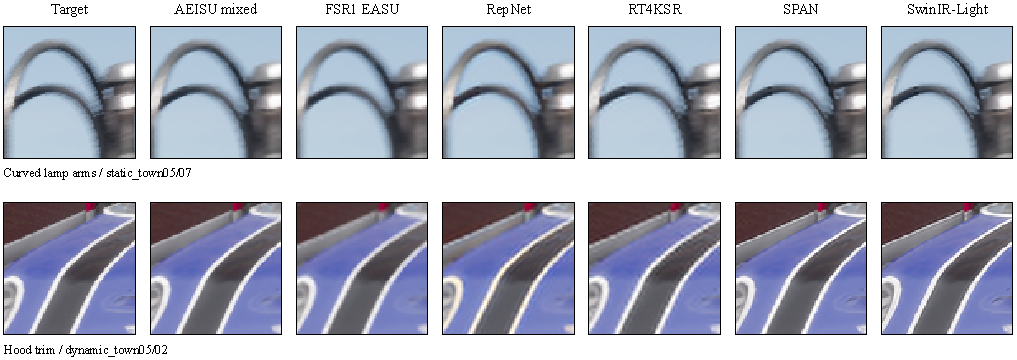
\includegraphics[width=0.98\textwidth]{figures/final_gameir_comparison_compact.pdf}
\caption{\textbf{External-method edge reconstruction.} Curved lamp arms and hood trim from GameIR Town05, static sequence 07 and dynamic sequence 02, frame 00000030~\cite{zhou2024gameir}. All methods use the same target-derived SSAA/area input and unchanged supplied HR reference. Matched $80\times80$ HR crops retain original colors and use nearest-neighbor enlargement. \model{} uses mixed FP8/FP16, EASU FP32, and neural comparators FP16. GameIR imagery derives from CARLA assets; attribution and license notices accompany the figures.}
\label{fig:external-edges}
\end{figure*}

We test Gaussian output smoothing ($\sigma=0.5,1,2$ HR pixels) on \model{} and EASU.
On Native, \model{} at $\sigma=1$ gains $0.646$ dB PSNR, while SSIM falls by $0.02058$ and LPIPS worsens by $0.14045$ (Fig.~\ref{fig:diagnostics}a).
Every tested setting worsens aggregate LPIPS on Native/FXAA/SMAA; on Area, the same grid lowers both PSNR and SSIM for both methods.
These differing metric responses illustrate the perception--distortion trade-off~\cite{blau2018tradeoff}; Supplementary Material, Section~S4.10 gives the complete sweep.

\begin{figure*}[t]
\centering
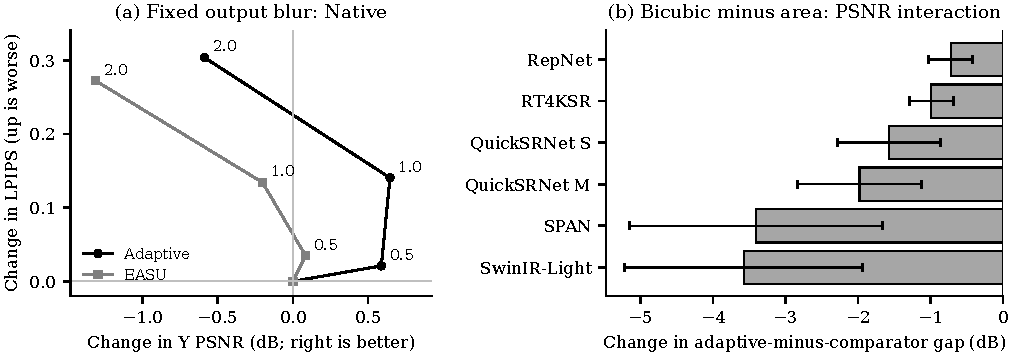
\includegraphics[width=0.98\textwidth]{figures/final_qrisp_diagnostics.pdf}
\caption{\textbf{Metric and degradation response.} (a) Changes from unblurred Native outputs under the fixed sigma grid; labels denote sigma in HR pixels. PSNR improves to the right, LPIPS worsens upward. (b) Change in the adaptive-minus-comparator Y PSNR gap when replacing area with bicubic inputs on the same references. Negative values favor the comparator's relative response. Bars show separate-family simultaneous 95\% bootstrap bands.}
\label{fig:diagnostics}
\end{figure*}

\subsection{Capacity and area-resolve agreement}
On Bicubic, all three metrics improve along the sequence from QuickSRNet Small to Medium, SPAN, and SwinIR.
This ordering changes on Native, and QuickSRNet Medium has lower PSNR than Small on the other four conditions.
RT4KSR has lower LPIPS than RepNet on area, bicubic, FXAA, and SMAA, but lower mean PSNR on most conditions.
The ordering therefore depends on the input degradation as well as model capacity.

Area-resolve agreement sorting narrows the Native adaptive-minus-EASU PSNR deficit from $0.742$ dB in the least-agreement stratum to $0.515$ dB in the most-agreement stratum.
Mean LR gradient energy is 2.53 times higher in the least-consistent group.
\model{}'s most-to-least PSNR separation is $5.91$ dB on Native but also $5.55$ dB on the common-reference area control.
Area-resolve agreement therefore captures image difficulty as well as rendering differences.
Stratum effects are descriptive because some extremes contain frames from only one sequence.
Subtracting each frame's Area adaptive-minus-EASU gap from its Native gap yields $-2.291$ dB overall (nominal interval $[-2.831,-1.756]$).
The adjusted point estimates are nearly unchanged across most-, middle-, and least-agreement strata ($-2.274$, $-2.334$, and $-2.266$ dB).

\subsection{Standard bicubic reconstruction}
\label{sec:classic-bicubic}
To evaluate the same architecture outside the game-capture setting, we train a separate checkpoint on the 800 official DIV2K training pairs with MATLAB-bicubic $2\times$ inputs~\cite{agustsson2017div2k}.
It uses RGB L1 loss for 3,000 epochs (915,000 updates), compared with 875,000 updates for the primary game-trained model.
Crop size, D4 augmentation, AdamW and fixed-offset stride-16 reconstruction gradients are unchanged; cosine decay from $2\times10^{-3}$ to $10^{-6}$ spans the full run.
Table~\ref{tab:classic-bicubic} reports dataset means over all 219 images in Set5~\cite{bevilacqua2012set5}, Set14~\cite{zeyde2011set14}, B100~\cite{martin2001bsd} and Urban100~\cite{huang2015urban100}, using the archived MATLAB-style bicubic pairs.
The original game-trained mixed deployment remains the model used in the QRISP and runtime studies.

% Generated by tools/paper_figures/classic_bicubic_results.py; numerical values from summary.json.
\begin{table*}[t]
\centering
\begingroup\fontsize{8}{9.5}\selectfont\setlength{\tabcolsep}{2.5pt}
\caption{Classic bicubic $2\times$ reconstruction. Dataset means of encoded-Y PSNR (P, dB), Y SSIM (S), and RGB LPIPS (L), after a two-HR-pixel border crop. All metrics are recomputed from RGB outputs. Both \model{} rows use the DIV2K L1 checkpoint trained for 3,000 epochs (915,000 updates): FP16 is the common FP16-controller/FP32-reconstruction path; mixed is the native FP8/FP16 deployment. Released comparators retain their recorded precision and training.}
\label{tab:classic-bicubic}
\begin{tabular}{l*{12}{r}}
\toprule
 & \multicolumn{3}{c}{Set5 (5)} & \multicolumn{3}{c}{Set14 (14)} & \multicolumn{3}{c}{B100 (100)} & \multicolumn{3}{c}{Urban100 (100)}\\
Method & P & S & L & P & S & L & P & S & L & P & S & L\\
\midrule
Bilinear &32.258&.91207&.17028&29.253&.84084&.23532&28.688&.81075&.30459&25.969&.80917&.24933\\
FSR1 EASU &33.865&.93130&.12233&30.457&.86763&.18344&29.572&.83950&.24733&27.208&.84594&.18840\\
FSRCNN &37.154&.95691&.05846&32.744&.90970&.10668&31.514&.89039&.16085&29.848&.90174&.10580\\
RepNet &35.848&.94509&.10667&32.003&.89427&.16634&30.907&.87172&.22500&28.800&.87967&.15645\\
RT4KSR &36.147&.95192&.06915&32.090&.90384&.12241&31.070&.88553&.18500&28.743&.88570&.13466\\
QuickSRNet S &37.195&.95756&.05686&32.834&.91064&.09947&31.616&.89244&.15133&30.179&.90671&.09428\\
QuickSRNet M &37.434&.95866&.05718&33.052&.91297&.09875&31.818&.89545&.14914&30.773&.91428&.08246\\
SPAN &38.099&.96102&.05556&33.706&.91914&.09537&32.235&.90058&.14743&32.212&.92924&.06570\\
SwinIR-Light &38.183&.96140&.05400&33.870&.92079&.08824&32.325&.90159&.14047&32.785&.93436&.05705\\
\midrule
\model{} FP16 &37.098&.95741&.06068&32.721&.91098&.10409&31.630&.89269&.15294&30.365&.90969&.08924\\
\model{} mixed &37.090&.95737&.06078&32.709&.91089&.10444&31.621&.89258&.15389&30.346&.90949&.08975\\
\bottomrule
\end{tabular}
\endgroup
\end{table*}


Both DIV2K precision variants have higher mean PSNR/SSIM and lower LPIPS than RepNet and RT4KSR on every set.
Relative to FSRCNN~\cite{dong2016fsrcnn}, the FP16 row's PSNR is lower by $0.056$ and $0.023$ dB on Set5 and Set14, but higher by $0.116$ and $0.517$ dB on B100 and Urban100; SSIM is higher on all four, and LPIPS is lower on the latter three.
Both variants exceed QuickSRNet Small on all three Urban100 metrics and on B100 PSNR/SSIM, although QuickSRNet Small has lower B100 LPIPS.
QuickSRNet Medium, SPAN and SwinIR-Light lead all three metrics on all four sets.
Native mixed-FP8/FP16 deployment lowers dataset-mean PSNR by $0.007$--$0.019$ dB and increases LPIPS by $0.00010$--$0.00095$ relative to the common FP16 path.
Supplementary Material, Section~S4.11, specifies mixed calibration and compares this run with the earlier 1,000-epoch MSE checkpoint.

\section{Implementation Measurements}
\label{sec:timing}
\label{sec:precision}
Native measurements use RTX 5090, batch one, CUDA graphs, and five trials of 100 warmup/200 measured iterations.
Median and p95 aggregate trial medians and within-trial p95 values.
The interval spans analysis through RGB reconstruction, after the input-fence wait and before output signaling; setup, decoding, capture, and presentation are outside it.
At 1080p input, halos/alignment pad processing to $1952\times1120$ before cropping.
The harness records hardware state without changing clock or power settings.

\begin{table}[h]
\centering\small
\caption{Resident GPU inference time (ms) on RTX 5090. Median and p95 are aggregated over five trials.}
\label{tab:latency}
\begin{tabularx}{\columnwidth}{Yrrrr}
\toprule
Input & FP16 & FP8 & Mixed & Mix. p95\\
\midrule
540p &0.285&0.204&0.132&0.152\\
720p &0.473&0.308&0.206&0.211\\
1080p &0.974&0.488&0.416&0.440\\
1440p &1.677&1.132&0.740&0.764\\
\bottomrule
\end{tabularx}
\end{table}

Mixed precision reduces median latency by 14.8\% relative to uniform FP8 at 1080p.
This gain combines datatype, fusion, conversion, and kernel-layout choices.
Uniform FP8 scales nonlinearly from 1080p to 1440p: $2.32\times$ latency for $1.78\times$ nominal input pixels.
Repeated stage measurements localize much of the excess to analysis/projection and the coefficient head (Supplementary Material, Section~S5.2).
The FP16 core uses Tensor Core WMMA; reconstruction uses conventional CUDA arithmetic.
The mixed runtime requires Blackwell SM120a and has been measured on RTX 5090.
Supplementary Material, Section~S5 gives runtime versions, instrumentation, and both timing geometries; expanded quality uses 540p-to-1080p.

\paragraph{Computational and implementation context.}
Table~\ref{tab:comparator-complexity} reports deployed parameters, counted MACs, and common FP16 PyTorch timings at the QRISP geometry.
The controller's 11,520 MACs/LR pixel exclude reconstruction: direct filter assembly adds 1,600 and RGB application adds 300, yielding 13,420 before analysis arithmetic and padding.
The common protocol uses batch-one full-frame channels-last tensors, cuDNN autotuning, disabled TF32, and five trials of 20 warmup/50 measured forwards, with eager and graph execution separated.
Under graph execution, QuickSRNet S takes $0.292$ ms and \model{} $1.588$ ms, whereas the optimized mixed deployment takes $0.132$ ms.
RepNet has fewer MACs and parameters, and its $0.129$ ms graph latency is close to the optimized \model{} latency.
Ordinary PyTorch synthesis materializes per-pixel filters and RGB patches; fused deployment avoids these image-sized intermediates.
Figure~\ref{fig:quality-latency} pairs current quality scores with fresh, backend-labeled timings.

\begin{table}[t]
\centering\small
\caption{Deployed complexity and FP16 PyTorch timing (ms), 540p-to-1080p. MACs count attention, required padding and AEISU reconstruction over the full padded PyTorch canvas; analysis and non-MAC operations are excluded. E: eager; G: graph replay.}
\label{tab:comparator-complexity}
\begin{tabularx}{\columnwidth}{Yrrrr}
\toprule
Method & Param. (k) & GMACs & E & G\\
\midrule
AEISU & 116.00 & 7.67 & 1.721 & 1.588\\
QuickSRNet S & 22.86 & 11.79 & 0.326 & 0.292\\
QuickSRNet M & 50.60 & 26.13 & 0.611 & 0.554\\
RepNet & 26.61 & 3.43 & 0.173 & 0.129\\
RT4KSR & 44.52 & 6.05 & 1.108 & 0.509\\
SPAN & 410.70 & 212.38 & 5.922 & 5.820\\
SwinIR-Light & 910.15 & 546.06 & 124.587 & 123.529\\
\bottomrule
\end{tabularx}
\end{table}


\begin{figure*}[t]
\centering
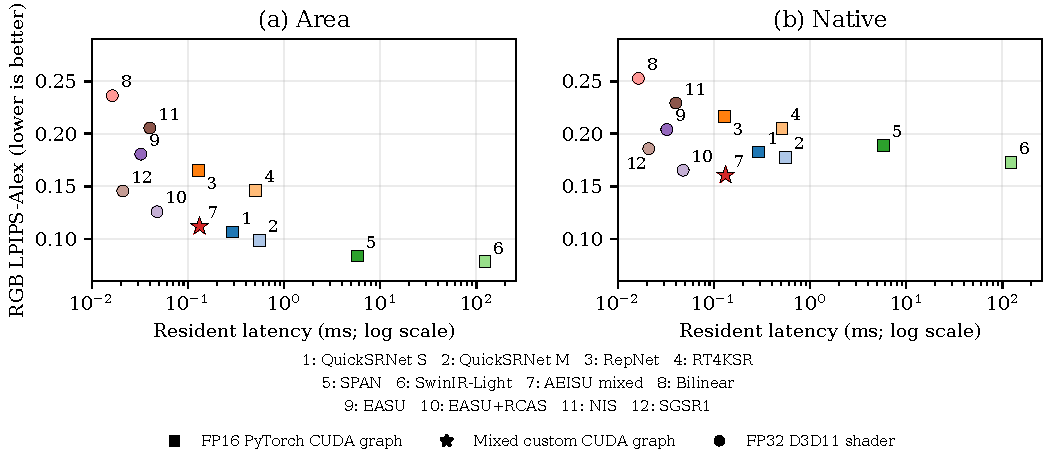
\includegraphics[width=0.98\textwidth]{figures/quality_latency_matched_geometry.pdf}
\caption{\textbf{Quality and implementation latency at 540p-to-1080p.} Current 600-pair Area and Native RGB LPIPS means are paired with fresh resident RTX 5090 timings. Symbols identify FP16 PyTorch graphs, the custom mixed CUDA graph, and FP32 D3D11 shaders. All timings use five trials; released-neural runs use 20 warmup/50 measured forwards and native/spatial runs use 100/200. Checkpoints, architectures, and shader identities were verified against the quality suite. Different numerical precision and backend optimizations prevent architecture-only speed conclusions.}
\label{fig:quality-latency}
\end{figure*}

Calibration uses 24 training and six separate calibration-validation images; details are in Supplementary Material, Section~S5.1.
On 219 area-derived natural images, mixed-to-FP32 output agreement averages $54.594$ dB RGB PSNR (minimum $31.658$ dB); target PSNR changes by $-0.0125$ dB on average.
The worst target RGB PSNR loss is $0.479$ dB; three images lose more than $0.1$ dB (Supplementary Material, Section~S5.1).

\paragraph{Conventional-CUDA deployment.}
A secondary deployment preserves the folded architecture and weights, using FP16 projection/refinement/head and INT8 compression, parallel-core, and expansion convolutions on conventional CUDA cores.
In a matched five-trial comparison, resident 1080p-to-4K latency is $1.275$ ms, versus $0.418$ ms for the native FP8/FP16 Tensor Core deployment, a $3.05\times$ latency ratio.
The latter session's $0.442$ ms p95 agrees closely with the repeated resolution sweep's $0.440$ ms.
Mean target Y PSNR decreases by $0.009$ dB on a 60-pair QRISP subset and $0.070$ dB on twelve internal 4K validation pairs.
This deployment comparison combines instruction path, precision, and fusion choices; detailed timing and quality results are in Supplementary Material.

\section{Ablation Studies}
\label{sec:ablation}
We examine output representation, learned analysis/base constants, parallel-core structure, coefficient clamping, and training degradation.
The architecture controls use separate 100-epoch runs; the degradation comparison uses two 1,000-epoch checkpoints, with one training run per configuration.
Each study evaluates final checkpoints with a common implementation within that study.
Training differences and their implications are summarized in Section~\ref{sec:limits} and specified in the supplement.

\begin{table*}[t]
\centering\small
\caption{Output-head quality and uniform-FP8 sensitivity: 60 QRISP AbandonedSchool Enhanced targets and 219 natural images, with area-derived inputs and uncropped Y metrics. Loss: FP16 minus FP8 target PSNR. Agreement: RGB PSNR between each model's FP8 and FP16 outputs.}
\label{tab:head-quality}
\begin{tabular}{llrrrrrr}
\toprule
Track & Head & \multicolumn{2}{c}{Y PSNR (dB)} & \multicolumn{2}{c}{Y SSIM} & Loss (dB) & Agreement (dB)\\
 & & FP16 & FP8 & FP16 & FP8 & & \\
\midrule
SSAA game & Adaptive & 32.874 & 32.823 & 0.90149 & 0.90083 & 0.051 & 49.81\\
 & RGB residual & 32.601 & 32.385 & 0.89709 & 0.89270 & 0.216 & 46.30\\
 & Depth-to-space & 32.119 & 31.012 & 0.88841 & 0.85247 & 1.107 & 35.84\\
\midrule
Natural images & Adaptive & 30.690 & 30.624 & 0.89737 & 0.89630 & 0.066 & 46.55\\
 & RGB residual & 30.327 & 30.160 & 0.89149 & 0.88503 & 0.167 & 43.83\\
 & Depth-to-space & 29.535 & 28.312 & 0.87818 & 0.82152 & 1.223 & 32.65\\
\bottomrule
\end{tabular}
\end{table*}

\begin{figure*}[t]
\centering
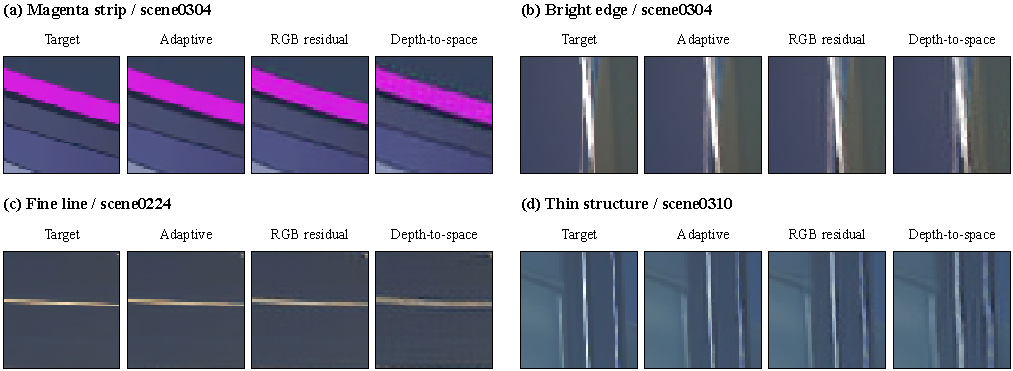
\includegraphics[width=0.98\textwidth]{figures/output_head_artifacts_compact.pdf}
\caption{\textbf{Output-head edge reconstruction.} UI-free \emph{Honkai: Star Rail} validation crops: (a) magenta strip, (b) bright edge, (c) fine line, (d) thin structure. Columns: target, adaptive filtering, RGB residuals, depth-to-space. Nearest-neighbor enlargement; original colors.}
\label{fig:head-artifacts}
\end{figure*}

\subsection{Output representation}
The backbone was developed under a strict below-input-resolution processing constraint before adaptive reconstruction was adopted.
We replace the head after the activated refinement tensor $F$ in Eq.~\eqref{eq:refine}, preserving the upstream architecture and training each variant end-to-end.
Let $\mathcal L_2(L;B_{\rm res})$ denote reconstruction by the residual model's learned four-phase $5\times5$ base, initialized to bilinear sampling.
Two minimal RGB alternatives are
\begin{align}
 \widehat T_{\rm res}&=\mathcal L_2(L;B_{\rm res})+
           \PS_4\big(C^1_{64\rightarrow48}(F)\big),\label{eq:reshead}\\
 \widehat T_{\rm direct}&=
           \PS_4\big(C^1_{64\rightarrow48}(F)\big).\label{eq:directhead}
\end{align}
Because $F$ is on the half-LR grid, the head must increase each spatial dimension by four to reach $2H\times2W$; hence $3\cdot4^2=48$ output channels.

The three tested heads are learned-base adaptive filtering, RGB residuals on a learned base, and direct depth-to-space RGB reconstruction without a base.
Each model was trained on the same 700 pairs for 100 epochs and 87,500 optimizer updates, with batch 32, HR patches of size 512, and cosine decay from $2\times10^{-3}$ to $10^{-6}$.
The coefficient and residual projections start at zero, giving their bilinear-initialized bases; the direct head starts at zero RGB.
The adaptive bank retains its sparse gradient estimator, while the direct heads use dense autograd.
The coefficient clamp in Eq.~\eqref{eq:coefficient-clamp} applies to the adaptive head.

\paragraph{Precision protocol.}
The FP8 stress test uses E4M3 weights and activations in all nine sequential convolutional stages; each of the four core stages contains two parallel convolutions, giving thirteen convolutions in total.
Weights have per-output-channel scales; activations have per-tensor scales.
Accumulation and learned reconstruction constants remain FP32, and native image I/O and linear-head outputs remain FP16.
All models use the same calibration images, procedure, and budget.
The RGB projections are zero-padded from 48 to 64 channels for native execution.



\paragraph{Quantization robustness.}
Adaptive filtering achieves higher FP16 reconstruction quality and smaller PSNR degradation under FP8 quantization on both datasets (Table~\ref{tab:head-quality}).
On QRISP SSAA, its FP16 Y PSNR exceeds residuals by $0.273$ dB and depth-to-space by $0.755$ dB.
FP8 reduces Y PSNR by $0.051$ dB, versus $0.216$ and $1.107$ dB, respectively.
Agreement between each model's FP8 and FP16 outputs follows the same ordering, indicating smaller numerical perturbations for adaptive filtering.
Supplementary Material, Section~S2 gives a coefficient-level mechanism consistent with the observation.

\paragraph{Haloing and edge reconstruction.}
\label{sec:head-artifacts}
Figure~\ref{fig:head-artifacts} shows narrower fringes for adaptive reconstruction in four selected validation regions, with the widest fringes in the depth-to-space output.
Faint fringing remains in the adaptive output.
The panels use FP16-AMP tiled outputs with matched crops and original colors.


\paragraph{Effect of the output representation.}
For 1080p input, the final feature tensor is at 540p.
Direct RGB heads must reconstruct fine structure from these compressed features.
The adaptive head instead conditions filters applied to original LR neighborhoods; the residual control samples LR through its base, but predicts the correction from half-LR features.
This distinction offers a plausible explanation for the observed fidelity and haloing differences on the shared backbone.
The tested adaptive configuration improves reconstruction without adding full-LR convolutional feature stages.

\subsection{Core architecture controls}
\label{sec:core-controls}
Three additional checkpoints freeze the analysis mixtures and stencils, freeze the bilinear-initialized base, or replace the parallel core with two dense $64$-channel convolutions.
Each uses the head study's 100-epoch recipe and seed 1234; the dense alternative matches Eq.~\eqref{eq:branchmac}'s bottleneck MACs.
All four use common FP16-controller/FP32-reconstruction evaluation on the frozen 600-pair sample.

\begin{table}[t]
\centering\small
\setlength{\tabcolsep}{3pt}
\caption{100-epoch core controls on Area. Training MSE is scaled by $10^4$; Y metrics and RGB LPIPS use 600 QRISP pairs and a two-HR-pixel crop. Lower LPIPS is better. The reference differs from the longer-trained mixed deployment.}
\label{tab:core-controls}
\begin{tabularx}{\columnwidth}{Yrrrr}
\toprule
Control & Train MSE & Y PSNR & Y SSIM & LPIPS\\
\midrule
Reference & 1.1471 & 31.297 & 0.91375 & 0.11390\\
Fixed inputs & 1.1506 & 31.304 & 0.91395 & 0.11219\\
Fixed bilinear base & 1.1566 & 31.283 & 0.91346 & 0.11395\\
Dense $64\times2$ core & 1.1578 & 31.277 & 0.91370 & 0.11396\\
\bottomrule
\end{tabularx}
\end{table}

Learning the analysis and base slightly lowers final training MSE, while external FP16 differences are small and metric-dependent (Table~\ref{tab:core-controls}).
Fixed inputs instead improve all three Bicubic metrics.
The parallel-core checkpoint has higher Area PSNR than the dense control by $0.020$ dB.
Under controller E4M3 rounding, the reference loses $0.038$ dB PSNR, versus $0.053$ for fixed inputs, $0.077$ for the fixed base and $0.075$ for the dense core.
Relative to the reference's precision change, the fixed base has greater LPIPS degradation and the dense core has greater SSIM and LPIPS degradation.
Supplementary Material, Section~S4, gives all-condition, RGB, and precision results.

\subsection{Coefficient clamp}
\label{sec:clamp-ablation}
An additional checkpoint replaces $g$ in Eq.~\eqref{eq:coefficient-clamp} with the identity, retaining the 100-epoch recipe and evaluating both checkpoints through common FP16-controller/FP32 tiled reconstruction on all 600 pairs.
Training MSE rises from $1.1471\times10^{-4}$ to $1.1664\times10^{-4}$.
Without the clamp, Area Y PSNR falls from $31.297$ to $31.253$ dB and Bicubic PSNR falls by $0.028$ dB; LPIPS also worsens on Bicubic and FXAA.
The exception is a small $0.006$ dB SMAA PSNR gain.
Under the core controls' uniform-controller E4M3 rounding test, Area PSNR loss increases from $0.038$ to $0.069$ dB, with an additional $0.032$ dB loss and greater LPIPS degradation.
Both typical and extreme raw coefficient magnitudes are larger without the clamp (Supplementary Material, Section~S4).

\subsection{Training degradation}
\label{sec:training-degradation}
With the same 1,000-epoch budget and targets, bicubic retraining raises Bicubic Y PSNR by $0.665$ dB but lowers Area and Native PSNR by $0.740$ and $0.718$ dB in common FP16 evaluation.
LPIPS improves on Area, Bicubic and FXAA.
The Bicubic run uses direct 8K-to-1080p resizing, whereas benchmark bicubic inputs are derived from HR targets (Supplementary Material, Section~S4).
On Bicubic, the retrained checkpoint reaches $31.725$ dB, still below SPAN ($32.598$) and SwinIR-Light ($32.876$), and also has higher LPIPS.

\section{Limitations and Discussion}
\label{sec:limits}
\model{} is single-frame and fixed at $2\times$, with $5\times5$ direct RGB reconstruction support.
Signed filters and an unconstrained base permit overshoot.
The profile diagnostic covers eligible isolated edges with approximately flat flanks; Native profiles also reflect differences between independently rendered LR/HR images.
Temporal stability and whole-image halo prevalence remain unevaluated.

All training controls use one seed.
The head study shares the backbone but varies initialization, gradient estimation, and constraints, and the degradation study uses different master/target resizing chains.
These differences limit attribution of the measured effects to individual design choices.
Repeated seeds and a full-LR feature-processing control would strengthen that attribution.

Primary training uses captures from two games and final-checkpoint selection without internal validation; the separate natural-image checkpoint uses DIV2K.
Incomplete scene-level acquisition records leave the overlap of existing same-game 4K diagnostic frames with training scenes unknown.
QRISP covers five environments with equally weighted agreement strata; released comparators retain their own training data and objectives.
The main quality study is 540p-to-1080p, while 1080p-to-4K evidence consists of timing and internal diagnostics.

The smoothing and agreement controls leave the contributions of aliasing, misalignment, rendering differences, and degradation specialization unresolved.
Runtime results apply to the evaluated implementations on one GPU and measure resident inference rather than application latency.
\begin{samepage}
\section{Conclusion}
We presented \model{}, a compact $2\times$ upscaler that predicts local filters below the input grid and applies them to original RGB samples.
The optimized mixed deployment reaches 0.416 ms median for resident 1080p-to-4K inference on RTX 5090.
Shared-backbone controls favor the tested adaptive head for reconstruction fidelity and FP8 robustness.
Area-resolved inputs are the model's strongest setting; its fidelity and LPIPS rankings change under bicubic and independently rendered inputs.\par
\end{samepage}

\paragraph{Supplementary material.}
The supplement and \href{https://github.com/AELabs42/AEISU}{companion repository} provide training and folding details, evaluation protocols, measurements, and visualizations; image corpora are excluded.

\begin{thebibliography}{99}
\fontsize{8}{9}\selectfont\raggedright
\setlength{\itemsep}{0.5pt}
\interlinepenalty=10000
\bibitem{dong2016srcnn}
C. Dong, C. C. Loy, K. He, and X. Tang.
Image Super-Resolution Using Deep Convolutional Networks.
\emph{IEEE TPAMI}, 38(2):295--307, 2016.
\href{https://arxiv.org/abs/1501.00092}{arXiv:1501.00092}.

\bibitem{shi2016espcn}
W. Shi, J. Caballero, F. Husz\'ar, J. Totz, A. P. Aitken, R. Bishop, D. Rueckert, and Z. Wang.
Real-Time Single Image and Video Super-Resolution Using an Efficient Sub-Pixel Convolutional Neural Network.
\emph{CVPR}, 2016.
\href{https://arxiv.org/abs/1609.05158}{arXiv:1609.05158}.

\bibitem{lim2017edsr}
B. Lim, S. Son, H. Kim, S. Nah, and K. M. Lee.
Enhanced Deep Residual Networks for Single Image Super-Resolution.
\emph{CVPR Workshops}, 2017.
\href{https://arxiv.org/abs/1707.02921}{arXiv:1707.02921}.

\bibitem{liang2021swinir}
J. Liang, J. Cao, G. Sun, K. Zhang, L. Van Gool, and R. Timofte.
SwinIR: Image Restoration Using Swin Transformer.
\emph{ICCV Workshops}, 2021.
\href{https://arxiv.org/abs/2108.10257}{arXiv:2108.10257}.

\bibitem{wan2024span}
C. Wan et al.
Swift Parameter-free Attention Network for Efficient Super-Resolution.
arXiv preprint, 2024.
\href{https://arxiv.org/abs/2311.12770v3}{arXiv:2311.12770v3}.

\bibitem{ren2024ntire}
B. Ren et al.
The Ninth NTIRE 2024 Efficient Super-Resolution Challenge Report.
\emph{CVPR Workshops}, pp. 6595--6631, 2024.
\href{https://arxiv.org/abs/2404.10343}{arXiv:2404.10343}.

\bibitem{romano2016raisr}
Y. Romano, J. Isidoro, and P. Milanfar.
RAISR: Rapid and Accurate Image Super Resolution.
2016.
\href{https://arxiv.org/abs/1606.01299}{arXiv:1606.01299}.

\bibitem{berger2023quicksrnet}
G. Berger, M. Dhingra, A. Mercier, Y. Savani, S. Panchal, and F. Porikli.
QuickSRNet: Plain Single-Image Super-Resolution Architecture for Faster Inference on Mobile Platforms.
\emph{CVPR Workshops}, pp. 2187--2196, 2023.
\href{https://arxiv.org/abs/2303.04336}{arXiv:2303.04336}.

\bibitem{mildenhall2018kpn}
B. Mildenhall, J. T. Barron, J. Chen, D. Sharlet, R. Ng, and R. Carroll.
Burst Denoising with Kernel Prediction Networks.
\emph{CVPR}, 2018.
\href{https://arxiv.org/abs/1712.02327}{arXiv:1712.02327}.

\bibitem{gharbi2017hdrnet}
M. Gharbi, J. Chen, J. T. Barron, S. W. Hasinoff, and F. Durand.
Deep Bilateral Learning for Real-Time Image Enhancement.
\emph{ACM Transactions on Graphics}, 36(4), Article 118, 2017.
\href{https://arxiv.org/abs/1707.02880}{arXiv:1707.02880}.

\bibitem{wu2018guided}
H. Wu, S. Zheng, J. Zhang, and K. Huang.
Fast End-to-End Trainable Guided Filter.
\emph{CVPR}, pp. 1838--1847, 2018.
\href{https://arxiv.org/abs/1803.05619}{arXiv:1803.05619}.

\bibitem{li2021lapar}
W. Li, K. Zhou, L. Qi, N. Jiang, J. Lu, and J. Jia.
LAPAR: Linearly-Assembled Pixel-Adaptive Regression Network for Single Image Super-Resolution and Beyond.
\emph{NeurIPS}, 2020.
\href{https://arxiv.org/abs/2105.10422}{arXiv:2105.10422}.

\bibitem{jia2017adaptive}
X. Jia, H. Chang, and T. Tuytelaars.
Super-Resolution with Deep Adaptive Image Resampling.
2017.
\href{https://arxiv.org/abs/1712.06463}{arXiv:1712.06463}.

\bibitem{jo2018duf}
Y. Jo, S. W. Oh, J. Kang, and S. J. Kim.
Deep Video Super-Resolution Network Using Dynamic Upsampling Filters Without Explicit Motion Compensation.
\emph{CVPR}, pp. 3224--3232, 2018.
\href{https://openaccess.thecvf.com/content_cvpr_2018/html/Jo_Deep_Video_Super-Resolution_CVPR_2018_paper.html}{CVF Open Access}.

\bibitem{ding2021repvgg}
X. Ding, X. Zhang, N. Ma, J. Han, G. Ding, and J. Sun.
RepVGG: Making VGG-style ConvNets Great Again.
\emph{CVPR}, 2021.
\href{https://arxiv.org/abs/2101.03697}{arXiv:2101.03697}.

\bibitem{zhou2024gameir}
L. Zhou, K. Han, N. Ling, W. Wang, and W. Jiang.
GameIR: A Large-Scale Synthesized Ground-Truth Dataset for Image Restoration over Gaming Content.
2024.
\href{https://arxiv.org/abs/2408.16866}{arXiv:2408.16866}.

\bibitem{nvidia2023gemm}
NVIDIA.
Matrix Multiplication Background User's Guide.
Deep Learning Performance documentation, accessed September 2026.
\href{https://docs.nvidia.com/deeplearning/performance/dl-performance-matrix-multiplication/index.html}{NVIDIA documentation}.

\bibitem{mercier2023qrisp}
A. Mercier, R. Erasmus, Y. Savani, M. Dhingra, F. Porikli, and G. Berger.
Efficient Neural Supersampling on a Novel Gaming Dataset.
\emph{ICCV}, 2023.
\href{https://arxiv.org/abs/2308.01483}{arXiv:2308.01483}.

\bibitem{conde2023repnet}
M.~V.~Conde, E.~Zamfir, R.~Timofte, et al.
Efficient Deep Models for Real-Time 4K Image Super-Resolution. NTIRE 2023 Benchmark and Report.
\emph{CVPR Workshops}, pp.~1495--1521, 2023.
RTVSR's RepNet contribution and \href{https://github.com/ezrealzhang/REPNet_NTIRE23-RTSR}{released implementation}.

\bibitem{zamfir2023rt4ksr}
E.~Zamfir, M.~V.~Conde, and R.~Timofte.
Towards Real-Time 4K Image Super-Resolution.
\emph{CVPR Workshops}, pp.~1522--1532, 2023.
\href{https://openaccess.thecvf.com/content/CVPR2023W/NTIRE/html/Zamfir_Towards_Real-Time_4K_Image_Super-Resolution_CVPRW_2023_paper.html}{CVF Open Access}.

\bibitem{amd2021fsr}
AMD GPUOpen.
FidelityFX Super Resolution 1: integration documentation and reference shaders.
\href{https://gpuopen.com/manuals/fidelityfx_sdk/techniques/super-resolution-spatial/}{GPUOpen integration manual}, accessed September 2026.

\bibitem{jimenez2012smaa}
J. Jimenez, J. I. Echevarria, T. Sousa, and D. Gutierrez.
SMAA: Enhanced Subpixel Morphological Antialiasing.
\emph{Computer Graphics Forum}, 31(2), 2012.
\href{https://www.iryoku.com/smaa/}{Paper and code}.

\bibitem{lottes2011fxaa311}
T. Lottes.
FXAA 3.11 in 15 Slides.
\emph{ACM SIGGRAPH course: Filtering Approaches for Real-Time Anti-Aliasing}, 2011.
\href{https://www.iryoku.com/aacourse/downloads/09-FXAA-3.11-in-15-Slides.pdf}{Course slides}.

\bibitem{basicsrmetrics}
XPixelGroup.
BasicSR: MATLAB-compatible color conversion and PSNR/SSIM metric implementation.
\href{https://github.com/XPixelGroup/BasicSR/blob/master/basicsr/utils/color_util.py}{Color utilities};
\href{https://github.com/XPixelGroup/BasicSR/blob/master/basicsr/metrics/psnr_ssim.py}{Metric source}, accessed September 2026.

\bibitem{mathworksresize}
MathWorks.
Resize an Image: antialiasing when shrinking an image.
\href{https://www.mathworks.com/help/images/resize-an-image.html}{MATLAB Image Processing Toolbox documentation}, accessed September 2026.

\bibitem{pharr2023pbrt}
M. Pharr, W. Jakob, and G. Humphreys.
\emph{Physically Based Rendering: From Theory to Implementation}, 4th edition.
MIT Press, 2023. Chapter 8, Sampling and Reconstruction.
\href{https://www.pbr-book.org/4ed/Sampling_and_Reconstruction/Image_Reconstruction}{Image reconstruction and pixel filters}.

\bibitem{nvidia2022nis}
NVIDIA.
NVIDIA Image Scaling SDK, version 1.0.3.
\href{https://github.com/NVIDIAGameWorks/NVIDIAImageScaling}{Official source repository}, accessed September 2026.

\bibitem{qualcomm2023gsr}
Qualcomm Snapdragon Game Studios.
Snapdragon Game Super Resolution 1.
\href{https://github.com/SnapdragonGameStudios/snapdragon-gsr/blob/main/sgsr/v1/README.md}{Official documentation}, accessed September 2026.

\bibitem{wang2004ssim}
Z. Wang, A. C. Bovik, H. R. Sheikh, and E. P. Simoncelli.
Image Quality Assessment: From Error Visibility to Structural Similarity.
\emph{IEEE Transactions on Image Processing}, 13(4):600--612, 2004.
\href{https://doi.org/10.1109/TIP.2003.819861}{doi:10.1109/TIP.2003.819861}.
\bibitem{zhang2018lpips}
R. Zhang, P. Isola, A. A. Efros, E. Shechtman, and O. Wang.
The Unreasonable Effectiveness of Deep Features as a Perceptual Metric.
\emph{CVPR}, 2018.
\href{https://arxiv.org/abs/1801.03924}{arXiv:1801.03924}.

\bibitem{blau2018tradeoff}
Y. Blau and T. Michaeli.
The Perception--Distortion Tradeoff.
\emph{CVPR}, 2018.
\href{https://arxiv.org/abs/1711.06077}{arXiv:1711.06077}.
\bibitem{agustsson2017div2k}
E. Agustsson and R. Timofte.
NTIRE 2017 Challenge on Single Image Super-Resolution: Dataset and Study.
\emph{CVPR Workshops}, 2017.
\href{https://openaccess.thecvf.com/content_cvpr_2017_workshops/w12/papers/Agustsson_NTIRE_2017_Challenge_CVPR_2017_paper.pdf}{CVF Open Access}.
\bibitem{bevilacqua2012set5}
M. Bevilacqua, A. Roumy, C. Guillemot, and M.-L. Alberi Morel.
Low-Complexity Single-Image Super-Resolution based on Nonnegative Neighbor Embedding.
\emph{BMVC}, pp. 135.1--135.10, 2012.
\href{https://doi.org/10.5244/C.26.135}{doi:10.5244/C.26.135}.
\bibitem{zeyde2011set14}
R. Zeyde, M. Elad, and M. Protter.
On Single Image Scale-Up Using Sparse-Representations.
\emph{Curves and Surfaces}, LNCS 6920, pp. 711--730, 2011.
\href{https://elad.cs.technion.ac.il/wp-content/uploads/2018/02/ImageScaleUp_LNCS.pdf}{Author manuscript}.
\bibitem{martin2001bsd}
D. Martin, C. Fowlkes, D. Tal, and J. Malik.
A Database of Human Segmented Natural Images and its Application to Evaluating Segmentation Algorithms and Measuring Ecological Statistics.
\emph{ICCV}, vol. 2, pp. 416--423, 2001.
\href{https://doi.org/10.1109/ICCV.2001.937655}{doi:10.1109/ICCV.2001.937655}.
\bibitem{huang2015urban100}
J.-B. Huang, A. Singh, and N. Ahuja.
Single Image Super-Resolution From Transformed Self-Exemplars.
\emph{CVPR}, pp. 5197--5206, 2015.
\href{https://openaccess.thecvf.com/content_cvpr_2015/html/Huang_Single_Image_Super-Resolution_2015_CVPR_paper.html}{CVF Open Access}.
\bibitem{dong2016fsrcnn}
C. Dong, C. C. Loy, and X. Tang.
Accelerating the Super-Resolution Convolutional Neural Network.
\emph{ECCV}, 2016.
\href{https://arxiv.org/abs/1608.00367}{arXiv:1608.00367}.
\end{thebibliography}
\end{document}
